% Definiciones y constantes de estilo
% Clase del documento
\documentclass[a4paper,12pt,twoside,openright,titlepage]{book}

%
% Paquetes necesarios
%

% Símbolo del euro
\usepackage{eurosym}
% Codificación UTF8
\usepackage[utf8]{inputenc}
% Caracteres del español
\usepackage[spanish]{babel}
% Código, algoritmos, etc.
\usepackage{listings}
% Definición de colores
\usepackage{color}
% Extensión del paquete color
\usepackage[table,xcdraw]{xcolor}
% Márgenes
\usepackage{anysize}
% Cabecera y pie de página
\usepackage{fancyhdr}
% Estilo título capítulos
%\usepackage{quotchap}
% Algoritmos (expresarlos mejor)
\usepackage{algorithmic}
% Citas mejoradas
\usepackage{cite}
% Títulos de secciones
\usepackage{titlesec}
% Fórmulas matemáticas
\usepackage[cmex10]{amsmath}
% Enumeraciones
\usepackage{enumerate}
% Páginas en blanco
\usepackage{emptypage}
% Separación entre cajas
\usepackage{float}
% Imágenes
\usepackage[pdftex]{graphicx}
% Mejora de las tablas
\usepackage{array}
% Mejora de los símbolos matemáticos
\usepackage{mdwmath}
% Separar figuras en subfiguras
\usepackage[caption=false,font=footnotesize]{subfig}
% Incluir pdfs externos
\usepackage{pdfpages}
% Mejoras sobre las cajas
\usepackage{fancybox}
% Apéndices
\usepackage{appendix}
% Marcadores (para el pdf)
\usepackage{bookmark}
% Estilo de enumeraciones
\usepackage{enumitem}
% Espacio entre líneas y párrafos
\usepackage{setspace}
% Glosario/Acrónimos
\usepackage[toc,xindy]{glossaries}

% Títulos de capítulo 
% http://osl.ugr.es/CTAN/macros/latex/contrib/titlesec/titlesec.pdf
\titleformat{\chapter}
{\normalfont\LARGE\bfseries}{\thechapter}{1em}{}

\titleformat{\section}
{\normalfont\Large\bfseries}{\thesection}{1em}{}

\titleformat{\subsection}
{\normalfont\large\bfseries}{\thesubsection}{1em}{}

% http://tex.stackexchange.com/questions/53338/reducing-spacing-after-headings
\titlespacing{\chapter}{0pt}{8pt plus 2pt minus 2pt}{4pt plus 2pt minus 2pt}
\titlespacing{\section}{0pt}{6pt plus 2pt minus 2pt}{2pt plus 2pt minus 2pt}
\titlespacing{\subsection}{0pt}{4pt plus 2pt minus 2pt}{0pt plus 2pt minus 2pt}

% Enlaces
\hypersetup{hidelinks,pageanchor=false,colorlinks,citecolor=Fuchsia,urlcolor=black,linkcolor=Cerulean}

% Euro (€)
\DeclareUnicodeCharacter{20AC}{\euro}

% Estilo de la bibliografía
\bibliographystyle{IEEEtran}

% Inclusión de gráficos
\graphicspath{{./graphics/}}

% Extensiones de gráficos
\DeclareGraphicsExtensions{.pdf,.jpeg,.jpg,.png}

% Definiciones de colores (para hidelinks)
\definecolor{LightCyan}{rgb}{0,0,0}
\definecolor{Cerulean}{rgb}{0,0,0}
\definecolor{Fuchsia}{rgb}{0,0,0}

% Keywords (español e inglés)
\def\keywordsEn{\vspace{.5em}
{\textbf{\textit{Key words ---}}\,\relax%
}}
\def\endkeywordsEn{\par}

\def\keywordsEs{\vspace{.5em}
{\textbf{\textit{Palabras clave ---}}\,\relax%
}}
\def\endkeywordsEs{\par}


% Abstract (español e inglés)
\def\abstractEs{\vspace{.5em}
{\textbf{\textit{Resumen ---}}\,\relax%
}}
\def\endabstractEs{\par}

\def\abstractEn{\vspace{.5em}
{\textbf{\textit{Abstract ---}}\,\relax%
}}
\def\endabstractEn{\par}

% Estilo páginas de capítulos
\fancypagestyle{plain}{
\fancyhf{}
\fancyfoot[CO]{\footnotesize\emph{\nombretrabajo}}
\fancyfoot[RO]{\thepage}
\renewcommand{\footrulewidth}{.6pt}
\renewcommand{\headrulewidth}{0.0pt}
}

% Estilo resto de páginas
\pagestyle{fancy}

% Estilo páginas impares
\fancyfoot[CO]{\footnotesize\emph{\nombretrabajo}}
\fancyfoot[RO]{\thepage}
\rhead[]{}

% Estilo páginas pares
\fancyfoot[CE]{\emph{\pieparcen}}
\fancyfoot[LE]{\thepage}
\fancyfoot[RE]{\pieparizq}
\lhead[]{}

% Guía del pie de página
\renewcommand{\footrulewidth}{.6pt}

% Nombre de los bloques de código
\renewcommand{\lstlistingname}{Código}

% Estilo de los lstlistings
\lstset{
    frame=tb,
    breaklines=true,
    postbreak=\raisebox{0ex}[0ex][0ex]{\ensuremath{\color{gray}\hookrightarrow\space}}
}

% Definiciones de funciones para los títulos
\newlength\salto
\setlength{\salto}{3.5ex plus 1ex minus .2ex}
\newlength\resalto
\setlength{\resalto}{2.3ex plus.2ex}

% Estilo de los acrónimos
\renewcommand{\acronymname}{Glosario}
\renewcommand{\glossaryname}{Glosario}
\pretolerance=2000
\tolerance=3000

% Pie de tabla
\addto\captionsspanish{
\def\tablename{Tabla}
\def\listtablename{\'Indice de tablas}
}

% Traducir appendix/appendices
\renewcommand\appendixtocname{Apéndices}
\renewcommand\appendixpagename{Apéndices}

% Comando code (lstlisting sin cambio de página)
\lstnewenvironment{code}[1][]%
  { \noindent\minipage{0.935\linewidth}\medskip
    \vspace{5mm}
    \lstset{basicstyle=\ttfamily\footnotesize,#1}}
  {\endminipage}

% Definiciones de comandos
\newcommand{\nombreautor}{Pablo Molins Ruano}
\newcommand{\nombretutor}{Pilar Rodríguez Marin}

% Descomentar si tu trabajo tiene un ponente
%\newcommand{\nombreponente}{TODO: Nombre del ponente}

\newcommand{\nombretrabajo}{Desarrollo de un sistema de cuestionarios adaptativos para el apoyo al aprendizaje}
\newcommand{\fecha}{Junio 2015}
\newcommand{\grado}{Grado en Ingeniería Informática}
\newcommand{\facultad}{Escuela Politécnica Superior}
\newcommand{\universidad}{Universidad Autónoma de Madrid}
\newcommand{\pieparizq}{\nombretrabajo}
\newcommand{\pieparcen}{Trabajo de Fin de Grado}
\newcommand{\logoizq}{Logo_EPS}
\newcommand{\logoder}{Logo_UAM}
\newcommand{\correo}{pablo.molins@estudiante.uam.es}

% Glosario y acrónimos
\makeglossaries
% Acrónimos

% TODO: Añadir aquí los acrónimos
% Ejemplo de acrónimo
\newacronym{FPGA}{FPGA}{Field-Programmable Gate Array}

% Glosario

% TODO: Añadir aquí las definiciones del glosario
% Ejemplo de glosario
\newglossaryentry{bitstream}{name={bitstream},description={En este contexto se refiere al binario que configura el Hardware de la FPGA}}

% Inicio del documento
\begin{document}

% Elección del idioma (español)
\selectlanguage{spanish}

%
% Portada
%
\pagenumbering{gobble}
%
% Portada
%

% Universidad, Facultad
\begin{titlepage}
\selectlanguage{spanish}
\begin{center}
\textbf{\begin{huge}
\universidad \\
\end{huge}}
\bigskip 
\begin{LARGE}
\facultad \\
\end{LARGE}
\end{center}

\bigskip
\bigskip

%
% Imágenes (logos) izquierdo y derecho
%
\begin{figure}[h]
	\begin{center}
		\includegraphics[scale=0.35]{\logoizq}
    	\hspace{1cm}
		\includegraphics[scale=0.4]{\logoder}
	\end{center}	
\end{figure}

\bigskip
\bigskip
\bigskip

% Grado
\begin{center}
\begin{large}
\textbf{\grado}\\
\end{large}
\end{center}

\bigskip

\textbf{\begin{center}
\begin{huge}
TRABAJO FIN DE GRADO
\end{huge}
\end{center}}

\bigskip
\bigskip

% Nombre del TFG
\begin{center}
\textbf{\begin{large}
\MakeUppercase{\nombretrabajo}\\
\end{large}}
\end{center}

% Nombre del autor...
\vspace{\fill}
\begin{center}
\textbf{\nombreautor}\\
%t ...tutor...
\textbf{Tutor: \nombretutor}\\
% ... y ponente, si está definido en main.tex
\ifcsname nombreponente\endcsname
\textbf{Ponente: \nombreponente}\\
\fi

\bigskip

% Fecha
\textbf{\MakeUppercase{\fecha}}\\
\end{center}
\end{titlepage}


\hypersetup{pageanchor=true}

%
% Resumen
%
\pagenumbering{Roman}
\setcounter{page}{0}
% Resumen en inglés
\chapter*{Abstract}

\begin{abstractEn}
TODO: Resumen en inglés, 250-500 palabras.

Lorem ipsum dolor sit amet, consectetur adipiscing elit. Aliquam malesuada libero auctor sapien volutpat, sed fringilla enim tristique. Aliquam varius lorem in risus tempus egestas. Aenean accumsan elementum diam vel commodo. Nulla lectus sapien, finibus ac mauris non, efficitur venenatis felis. Donec at rutrum dolor, a lobortis arcu. In fermentum hendrerit bibendum. Phasellus eget arcu quam. Maecenas vulputate sapien eu dictum pulvinar. Suspendisse sit amet neque a turpis efficitur dapibus ut et turpis.

Vestibulum commodo faucibus tellus vitae consequat. Donec purus enim, hendrerit vitae feugiat sed, sagittis in tortor. Duis sed ex non ligula cursus dapibus. Etiam pellentesque suscipit dolor, vel facilisis est ornare sed. Nullam eleifend tellus non elementum efficitur. Donec semper felis ac porttitor ultricies. Vestibulum sodales justo nisl, in egestas lacus egestas nec. Fusce faucibus felis lacus, sit amet placerat justo porta vitae. Nullam volutpat viverra lorem quis euismod. Duis felis erat, dictum et sem vitae, fringilla ultrices dui. Morbi mattis arcu at orci accumsan facilisis. Aenean tortor velit, hendrerit id vulputate ac, sagittis nec libero. Donec elementum dolor orci, a mattis augue lobortis nec. Suspendisse vulputate, diam vel accumsan pellentesque, ex purus volutpat ipsum, vel luctus urna sem non turpis. Donec vitae molestie odio.

Donec lobortis, eros non sodales dapibus, ex eros sollicitudin tortor, ut vulputate massa nibh sit amet ipsum. Sed a lectus eu diam pretium vestibulum. Pellentesque finibus, felis ac finibus vulputate, libero mauris placerat nulla, ut vestibulum ante metus ut neque. Aliquam tempus tortor ac mauris pulvinar iaculis. Vivamus pretium id libero sed tempus. Donec tincidunt turpis tempor vehicula egestas. Vestibulum elementum, urna non tincidunt tempus, risus ipsum posuere felis, ac suscipit diam nunc et neque. Vestibulum faucibus leo vel nibh tempor tincidunt. Nullam nunc augue, aliquet in congue nec, gravida at risus. Proin semper iaculis nisi vitae imperdiet. Suspendisse sed risus feugiat, dapibus sapien quis, pulvinar turpis.

Maecenas convallis aliquet euismod. Donec sollicitudin ligula nec lorem dignissim, sit amet finibus felis mollis. Fusce eget sapien eu sapien blandit congue quis a odio. Fusce accumsan condimentum dapibus. Aliquam eu ante porttitor nulla pellentesque feugiat pharetra nec mauris. Ut tincidunt urna vitae ligula mattis malesuada. Interdum et malesuada fames ac ante ipsum primis in faucibus. Integer pretium tincidunt nisi, in pulvinar velit dapibus et.
\end{abstractEn}

% Palabras clave en inglés
\begin{keywordsEn}
TODO: Palabras clave en inglés, separadas por coma.
\end{keywordsEn}

% Resumen en español
\chapter*{Resumen}

\begin{abstractEs}
TODO: Resumen en español, 250-500 palabras.

Lorem ipsum dolor sit amet, consectetur adipiscing elit. Aliquam malesuada libero auctor sapien volutpat, sed fringilla enim tristique. Aliquam varius lorem in risus tempus egestas. Aenean accumsan elementum diam vel commodo. Nulla lectus sapien, finibus ac mauris non, efficitur venenatis felis. Donec at rutrum dolor, a lobortis arcu. In fermentum hendrerit bibendum. Phasellus eget arcu quam. Maecenas vulputate sapien eu dictum pulvinar. Suspendisse sit amet neque a turpis efficitur dapibus ut et turpis.

Vestibulum commodo faucibus tellus vitae consequat. Donec purus enim, hendrerit vitae feugiat sed, sagittis in tortor. Duis sed ex non ligula cursus dapibus. Etiam pellentesque suscipit dolor, vel facilisis est ornare sed. Nullam eleifend tellus non elementum efficitur. Donec semper felis ac porttitor ultricies. Vestibulum sodales justo nisl, in egestas lacus egestas nec. Fusce faucibus felis lacus, sit amet placerat justo porta vitae. Nullam volutpat viverra lorem quis euismod. Duis felis erat, dictum et sem vitae, fringilla ultrices dui. Morbi mattis arcu at orci accumsan facilisis. Aenean tortor velit, hendrerit id vulputate ac, sagittis nec libero. Donec elementum dolor orci, a mattis augue lobortis nec. Suspendisse vulputate, diam vel accumsan pellentesque, ex purus volutpat ipsum, vel luctus urna sem non turpis. Donec vitae molestie odio.

Donec lobortis, eros non sodales dapibus, ex eros sollicitudin tortor, ut vulputate massa nibh sit amet ipsum. Sed a lectus eu diam pretium vestibulum. Pellentesque finibus, felis ac finibus vulputate, libero mauris placerat nulla, ut vestibulum ante metus ut neque. Aliquam tempus tortor ac mauris pulvinar iaculis. Vivamus pretium id libero sed tempus. Donec tincidunt turpis tempor vehicula egestas. Vestibulum elementum, urna non tincidunt tempus, risus ipsum posuere felis, ac suscipit diam nunc et neque. Vestibulum faucibus leo vel nibh tempor tincidunt. Nullam nunc augue, aliquet in congue nec, gravida at risus. Proin semper iaculis nisi vitae imperdiet. Suspendisse sed risus feugiat, dapibus sapien quis, pulvinar turpis.

Maecenas convallis aliquet euismod. Donec sollicitudin ligula nec lorem dignissim, sit amet finibus felis mollis. Fusce eget sapien eu sapien blandit congue quis a odio. Fusce accumsan condimentum dapibus. Aliquam eu ante porttitor nulla pellentesque feugiat pharetra nec mauris. Ut tincidunt urna vitae ligula mattis malesuada. Interdum et malesuada fames ac ante ipsum primis in faucibus. Integer pretium tincidunt nisi, in pulvinar velit dapibus et.
\end{abstractEs}

% Palabras clave en español
\begin{keywordsEs}
TODO: Palabras clave en español, separadas por coma.
\end{keywordsEs}

%
% Agradecimientos
%
\chapter*{Agradecimientos}

Este trabajo no hubiera sido posible sin que hace tres años Sacha y Pilar me dejaran jugar con ellos. Quiero creer que gracias a ello ahora soy un poco menos ``yogurín''. Gracias a Sacha por brindarme esta oportunidad y haberme empujado estos años y a Pilar por su impagable consejo, ayuda y paciencia.

También quiero dar las gracias a Covadonga Sevilla, Francisco L. Borrego, Santiago Atrio y Simone Santini por haber accedido a utilizar e-valUAM en sus clases. Así mismo, gracias (o perdón) a todos los alumnos de las asignturas de ``Historia Antigua I'' del Grado en Historia, ``El Entorno como Instrumento Educativo'' del Grado en Educación Infantil, ``Proyecto de Programación'' del Doble Gradon en Informática y Matemáticas y ``Diseño y Análisis de Algoritmos'' del Grado y Doble Grado en Ingeniería Informática.

Gracias a mis compañeros de carrera, con los que estos cuatro años se han hecho mucho más divertidos: Álvaro, Dani, Diego, Euler, Isa, José, Julian, María, Miguel, Mónica y Rober. Gracias a los compañeros que traje de antes, aún conservo y tanto me han acompañado. Gracias también a todos los grandes profesores con los que he tenido el placer de aprender estos cuatro años.

Por último, gracias a mis padres y a mi increible hermana Lucía.



% Cita
\begin{flushright}
\textit{%<<I often liked to play tricks on people when I was at MIT. One time, in mechanical drawing class, some joker picked up a French curve (a piece of plastic for drawing somooth curves--–a curly, funny-looking thing) and said ``I wonder if the curves on this thing have some special formula?''\\
%I thought for a moment and said ``Sure they do. The curces are very special curves. Lemme show ya,'' and I picked up my French curve and began to turn it slowly. ``The French curve is mado so that at the lowest point on each curve, no matter how you turn it, the tangent is horizontal.''\\
%All the guys in the class were holding their French curve up at different angles, holding their pencil up to it at the lowest point and laying it along, and discovering that, sure enough, the tangent is horizontal. They were all excited by this ``discovery''---even though they hal already gone through a certain amount of calculus and had already ``learned'' that the derivate (tangent) of the minumen (the lowest point) of \emph{any} curve is zero (horizontal). They didn't put two and two together. They didn't even know what they ``knew.''\\
``I don`t know what's the matter with people: they don't learn by understanding; they learn by some other way---by rote or something. Their knowledge is so fragile!''\\}
Richard P. Feynman. ``Surely you're joking, Mr. Feynman!''
\end{flushright}

  

%
% Tabla de contenidos
%
\tableofcontents
\listoftables
\listoffigures


%
% Glosario
%
\printglossary[title=Glosario,toctitle=Glosario]
\cleardoublepage


% Estilo de párrafo de los capítulos
\setlength{\parskip}{0.75em}
\renewcommand{\baselinestretch}{1.25}
% Interlineado
\spacing{1.3}
% Numeración contenido
\pagenumbering{arabic}
\setcounter{page}{1}

%
% Introducción
%
\pagenumbering{arabic}
\setcounter{page}{1}
\chapter{Introducción \label{sec:introduccion}}

En esta sección se detallará qué ha motivado la realización de este Trabajo Fin de Grado. A continuación, se explicará en qué marco se ha llevado a cabo, así como el alcance del proyecto, especificando sus objetivos. Por último, se expondrá  la estructura que sigue el resto del presente documento.

\section{Motivación}

%\textbf{¿Por qué son necesarios los test adaptativos?
%¿Qué puede aportar un sistema informático a los test adaptativos?
%¿Dónde se pueden utilizar?
%Listar ejemplos: MOOCs, AEH, educación clásica, contextos donde el usuario no dispone de conocimiento informático.}

La revolución que ha supuesto la introducción de las tecnologías informáticas en cada día más aspectos de la vida humana es una revolución de un profundo calado. La informática ha traído consigo mejoras inconmensurables en las comunicaciones, la automatización o el desarrollo científico (por citar solo algunos ejemplos) que, en general, han permitido al ser humano librarse de tareas repetitivas y dedicar más esfuerzo a las tareas verdaderamente interesantes.

La educación ha bebido de los avances en informática pero a un ritmo mucho menor que otras áreas, a pesar de ser uno de los pilares sociales. Aunque cada día es más habitual el aprendizaje asistido por tecnologías, \acrshort{TEL}, con el uso de ordenadores en las aulas, Internet como recurso docente o pizarras digitales en las aulas, \textbf{gran parte de la actividad educativa ha permanecido inalterada, anclada en modelos artesanales}. Por ejemplo, la evaluación de los alumnos a día de hoy se sigue basando principalmente en cuestionarios creados cada año, que los alumnos responden en papel y los profesores corrigen a mano, uno a uno.

\textbf{La evaluación artesanal de los alumnos conlleva problemas}. Por un lado, al crearse cada año un nuevo conjunto de preguntas es posible que haya alguna pregunta mal planteada que no se descubra hasta la corrección. Así mismo, la cantidad ingente de tiempo que pierden los profesores en crear y corregir los exámenes es tiempo que no dedican a explicar a los alumnos temario, reforzar las partes más complicadas o a responder dudas. Ese tiempo también se traduce en que los alumnos sufran retrasos a la hora de recibir retroalimentación sobre su empeño, una información que es muy valiosa y de la que cuanto antes dispongan, mejor.

La aparición recientemente de nuevas líneas de investigación en educación y tecnologías, como los \acrshort{MOOC} o los \acrshort{SPOC}, demuestran que \textbf{existe interés en el tema y campos donde realizar mejoras}.

De todos esos posibles campos donde la educación y las tecnologías pueden encontrarse, \textbf{este trabajo se centra en la parte de la evaluación del conocimiento}, tanto como herramienta del estudiante para medir su desempeño como herramienta del docente para conocer el estado de sus alumnos. En ambos casos, esa información puede resultar clave. Hoy en día, aún en muchos casos, el alumno obtiene retroalimentación solo una vez por asignatura y justo al final, cuando ya no puede rectificar. En el mejor de los casos, el alumno tendrá uno o dos exámenes parciales, que le darán algo de información antes de que sea demasiado tarde, pero será a costa de un mayor esfuerzo del profesor.

Creyendo que la tecnología puede aportar mucho al proceso de evaluación, en este trabajo \textbf{se presenta una propuesta de un sistema adaptativo orientado a crear cuestionarios que sirvan de apoyo al aprendizaje, ya sea como sistema de autoevaluación de los alumnos o sistema de evaluación para los docentes.} 
Buscando que sea útil en la mayor cantidad de áreas del conocimiento y  contextos posibles, se ha creado para que sea fácil de usar, sin importar los conocimientos informáticos del usuario. 

Así mismo, buscando que ahorre tiempo al profesorado, se ha creado un sistema que permite fácilmente crear nuevos cuestionarios, que se evalúen automáticamente y que vayan acompañados de un análisis de los resultados automático. Con ello se busca también que el docente pueda detectar lo más rápido posible las lagunas en sus alumnos y mejorar así ambos en su empeño.


%Algunas nuevas invenciones, como los \acrshort{MOOC} demuestran que el aprendizaje asistido por tecnologías, \acrshort{TEL}, es un área donde aún queda trabajo y en múltiples facetas. Este Trabajo 

%Desde su creación, los ordenadores han sido introducidos de forma progresiva en cada vez más sectores, con grandes beneficios. La educación es un ejemplo de ello, aunque aún todavía es un ejemplo incompleto. El aprendizaje asistido por tecnologías, \acrshort{TEL}, y en concreto, el aprendizaje asistido por ordenador, \acrshort{CAL}, es cada vez más habitual y ha sido aplicada con éxito a la educación presencial, semipresencial o a distancia, aportando grandes ventajas en cada modalidad. La reciente aparición y popularización de los \acrshort{MOOC} ha vuelto a demostrar la necesidad de seguir ampliando estas áreas {CITA}.

%Dentro de las \acrshort{CAL} una de las ramas de interés es la conocida como tests adaptativos por ordenador, o \acrshort{CAT}. Los \acrshort{CAT} se han utilizado para múltiples propósitos, como puntuación instantánea \cite{Wainer00}, la mejora de  competencias lingüísticas \cite{Chapelle06} , identificación de estilos de aprendizaje \cite{Ortigosa10}, la habilidad matemática \cite{Klinkenberg11}, o la evaluación del estado de salud \cite{Revicki97}.

%\textbf{¿Cuál ha sido exactamente el trabajo? ¿Motivación? Creo que no ¿e-valUAM? Sí ¿Modelo de estudiantes? Sí ¿Protocolo para crear las preguntas? También ¿Exámenes con duda? Sí.}

% sirve para múltiples objetivos, como aumentar la motivación de los alumnos {CITA}, sus resultados académicos {CITA} o su }}

\section{Marco y antecedentes}

%En qué investigación se engloba el proyecto. ¿Citar financiación?

Durante el curso académico 2011/2012 empezó una colaboración entre miembros de la Escuela Politécnica Superior y la Facultad de Filosofía y Letras, ambas de la Universidad Autónoma de Madrid. Gracias a dicha colaboración, durante los cursos 11/12 y 12/13 se llevaron a cabo varias experiencias en las que alumnos de los Grados en Ingeniería Informática e Historia colaboraban en la creación de videojuegos como método docente altamente motivador  \cite{Sevilla12}\cite{Molins14Videogames}.

De estas primeras experiencias surgió un grupo interdisciplinar interesado en la introducción de las tecnologías en el proceso docente. Durante finales del curso 12/13 se decidió explorar nuevas posibilidades, esta vez centrándose en los cuestionarios adaptativos utilizados para la evaluación. En ese momento fue cuando surgió la línea de investigación en la que ha estado enmarcado este TFG. 

Durante el verano de 2013 se empezaron a definir los primeros modelos de usuario y de adaptación, que se plasmarían en un primer prototipo del sistema desarrollado para el curso 13/14. Dicho modelo se utilizó en una asignatura del Grado de Historia durante el curso 13/14.

Con la incorporación al grupo de profesores de la Facultad de Formación de Profesorado y Educación, también de la UAM, se inició el desarrollo de un segundo prototipo que se utilizó, esta vez, en una asignatura del Grado en Magisterio en Educación Infantil, explorando nuevos modelos, nueva funcionalidad y en un entorno con más usuarios.

Esta investigación ha sido apoyada por la Convocatoria de Proyectos de Innovación Docente de la Universidad Autónoma de Madrid durante los cursos 2012/2013, 2013/2014, y 2014/2015, y por una Beca de Colaboración del Ministerio de Educación, Cultura y Deporte para el curso 2014/2015.

\section{Alcance y objetivos}

%¿Qué pretende lograr el sistema?
%¿Qué NO pretende lograr el sistema?

Dentro de la línea de investigación en la que se engloba el proyecto, \textbf{este Trabajo Fin de Grado se ha centrado exclusivamente en la parte técnica del mismo}. Para probar las hipótesis planteadas durante la investigación desde el principio se entendió como \textbf{necesario crear un sistema online que implementara los modelos que se querían probar}, para que pudiera ser utilizado en experiencias reales y de ahí obtener resultados con los que analizar las hipótesis. Así, este TFG tiene como sus objetivos:

\begin{itemize}
	\item Disponer de un sistema que \textbf{permita a profesores crear cuestionarios online} para que sean utilizados como herramienta de autoevaluación por los alumnos o como parte de una evaluación por parte del docente.
	\item Que sea un sistema que puedan utilizar profesores y alumnos de \textbf{múltiples áreas del conocimiento, sin que necesiten conocimientos informáticos avanzados.}
	\item Habilitar para el profesor \textbf{herramientas de análisis} que le permitan detectar rápidamente las deficiencias que puedan existir en las preguntas  elaboradas o en el conocimiento de los alumnos.
	\item Desarrollar un \textbf{sistema web robusto ante los picos de demanda} que suponen todos los alumnos de un curso accediendo a la vez durante un examen.
	\item Crear un \textbf{modelo de datos que abstraiga las entidades y relaciones de una evaluación}, que permita guardar toda la información posible para realizar análisis posteriores.
	\item Diseñar una \textbf{arquitectura para el sistema que sea flexible} y permita incorporar los nuevos modelos que se van a ir desarrollando con la investigación.
\end{itemize}

% Hablar de qué no cubre el sistema


\section{Estructura del documento}

En el siguiente capítulo, sobre el estado del arte, se presenta un repaso a la evolución de los cuestionarios adaptativos por ordenador, además de una introducción a las características de los sistemas que a día de hoy están siendo desarrollados. 

A continuación, se presenta un capítulo dedicado a las fases de análisis, diseño y desarrollo de la solución propuesta. En este capítulo se detalla la metodología de proyecto elegida, el análisis de requisitos (funcionales y no funcionales), además de la división del sistema en módulos y cómo se han implementado todos ellos.

En el cuarto capítulo, el dedicado a las pruebas y resultados, se exponen los resultados obtenidos con cada uno de los dos prototipos desarrollados, explicando los entornos reales donde se probaron, además de cuál fue su desempeño.

El siguiente capítulo expone las conclusiones del trabajo. Por último, se dedica un capítulo a trabajo futuro, seguido de la bibliografía y una serie de apéndices. % TODO: Detallar los apéndices.

% Cuatro líneas. Resumir todo el trabajo. Ir haciéndolo
%
% Estado del arte
%
\chapter{Estado del Arte\label{sec:estado_del_arte}}

A lo largo de toda la historia de la evaluación se ha buscado el equilibrio entre exámenes individuales y colectivos. En un examen individual se puede lograr una batería de preguntas en las que no haya ninguna inapropiada y asegurar que el evaluado entiende correctamente la tarea. En los exámenes colectivos se asegura que la evaluación ha sido uniforme para todos los evaluados, a la vez que se reduce enormemente el coste de evaluar \cite{Wainer00}.

Durante la década de los setenta aparecieron los primeros trabajos que exploraban la posibilidad de crear exámenes administrados masivamente pero adaptados a los individuos, eligiendo las nuevas preguntas en función de las respuestas anteriores, con el objetivo de buscar la manera óptima de evaluar al individuo en cuestión \cite{Lord68}. Desde un principio fue evidente que este nuevo tipo de evaluación solo sería posible gracias a los ordenadores, por lo que pasó a conocerse como \textit{Computerized Adaptive Testing}, o \acrshort{CAT}.

Entre las mejoras que prometían los \acrshort{CAT} destacaban las siguientes \cite{Green83}:

\begin{enumerate}
	\item \textbf{Aumentan la seguridad de los test}, ya que se almacena un conjunto de preguntas y no solo aquellas preguntas que especificamente se van a realizar. Así, si alguien obtiene acceso a las preguntas no puede mejorar su nota sencillamente estudiando unas cuantas (solo podría mejorar su nota estudiando un porcentaje muy elevado de las preguntas, en cuyo caso se ha ganado esa buena nota).
	\item \textbf{Cada persona puede realizar el examen a su ritmo}, abriendonos a más estilos de respuesta. Además, \texbf{se puede conocer el tiempo que ha tardado en responderse cada pregunta}, información que puede ser útil para evaluar.
	\item \textbf{A todo el mundo se le presenta un reto, sin que nadie se desaliente}. A cada individuo se le presenta las preguntas del rango de dificultad más adecuado para él.
	\item \textbf{Los problemas asociados con el carácter físico de las hojas de respuestras tradicionales desaparecen}. No existe ambigueadad en respuestas a medio marcar o medio borrar, la perdida de la hoja o las dudas sobre lo que está escrito en la hoja.
	\item \textbf{El examen puede ser corregido inmediatamente}, reduciendo el tiempo que el alumno tiene que esperar para obtener retroalimentación, lo cual es especialmente útil en los exámenes dirigidos a ser utilizados para autoevaluación.
	\item \textbf{Facilita realizar un precalibrado de los test}, ya que el sistema puede ir introduciendo discretamente nuevas preguntas para ser calibradas.
	\item \textbf{Se pueden eliminar inmediatamente preguntas defectuosas.}
	\item Una enorme variedad de \textbf{nuevos formatos de preguntas pueden ser explorados}. El sistema de respuesta múltiple no es el único válido. Se pueden crear problemas aritméticas a las que deba introducirse una respuesta numérica. La memoria podría ser evaluada utilizando múltiples marcos. Utilizando sintetizadores de voz, se pueden hacer exámenes de ortografía. Se pueden utilizar vídeos para sustituir largas explicaciones en exámenes de juicio situacional.
\end{enumerate}

Desde entonces, los \acrshort{CAT} se han utilizado con éxito para múltiples propósitos, como puntuación instantánea \cite{Wainer00}, la mejora de competencias lingüísticas \cite{Chapelle06} , identificación de estilos de aprendizaje \cite{Ortigosa10}, la habilidad matemática \cite{Klinkenberg11}, o la evaluación del estado de salud \cite{Revicki97}. Así mismo, se ha comprobado que los sistemas educativos que dan retroalimentación inmediata a los alumnos son más efectivos que estrategias de aprendizaje clásicas\cite{Kumar04}. 

A pesar de todas las ventajas que ofrecen, los \acrshort{CAT} han presentado algunos incovenientes que deben ser tratados, aunque múltiples investigaciones han hecho importantes avances. Destacan los siguientes \cite{Wainer00}:

\begin{enumerate}
 	\item Nuevos modelos de exámen requieren crear nuevas teorías psicométricas. Para el caso de los \acrshort{CAT} ha sido bastante utilizada la \textit{Item Response Theory}, o \acrshort{IRT}. La \acrshort{IRT} es un modelo matemático que caracteriza qué ocurre cuando un individuo se encuentra con un pregunta. Cada individuo es caracterizado por un valor de competencia y cada pregunta por una dificultad y se busca elegir la mejor pregunta en función de esos dos valores\cite{Wainer83}.
	\item Los \acrshort{CAT} requieren de una extensa bateria de preguntas, lo que hace compliada \textbf{la correcta calibración de las preguntas}. La estrategia más común para asegurar un buen proceso de calibración implica que la bateria sea provada por una amplia población \cite{Klinkenberg11}. Sin embargo, dado que el pre-calibrado no siempre es posible, se utilizan modelos de estudiantes con el fin de perfeccionar la calidad de la estrategia de evaluación \cite{Antal11}\cite{Galvez09}\cite{Molins14Test}.
	\item En los entornos \acrshort{CAT} hay tres preguntas clave:
	\begin{enumerate}
		\item ¿Cómo se determina con qué pregunta empieza el test?
		\item ¿Cómo se determina la siguiente pregunta que debe plantearse una vez hemos visto la respuesta del examinado a la pregunta actual?
		\item ¿Cómo se determina cuándo parar el test?
	\end{enumerate}
	La elección de la respuesta a estas tres preguntas no es trivial ni única. Existen muchos algoritmos de comienzo, continuación y parada y al ser tres partes claves del flujo que sigue todo \acrshort{CAT} (como se puede ver en la figura \ref{fig:diagrama_flujo_CAT}), la mínima variación en cualquiera de ellos genera sistemas muy distintos. Cada nuevo modelo que aporte un nueva versión de los tres algoritmos necesita ser probado para asegurar su confiabiliad, precisión y validez\cite{Wainer00}.
\end{enumerate}

\begin{figure}[htp!]
	\centering
	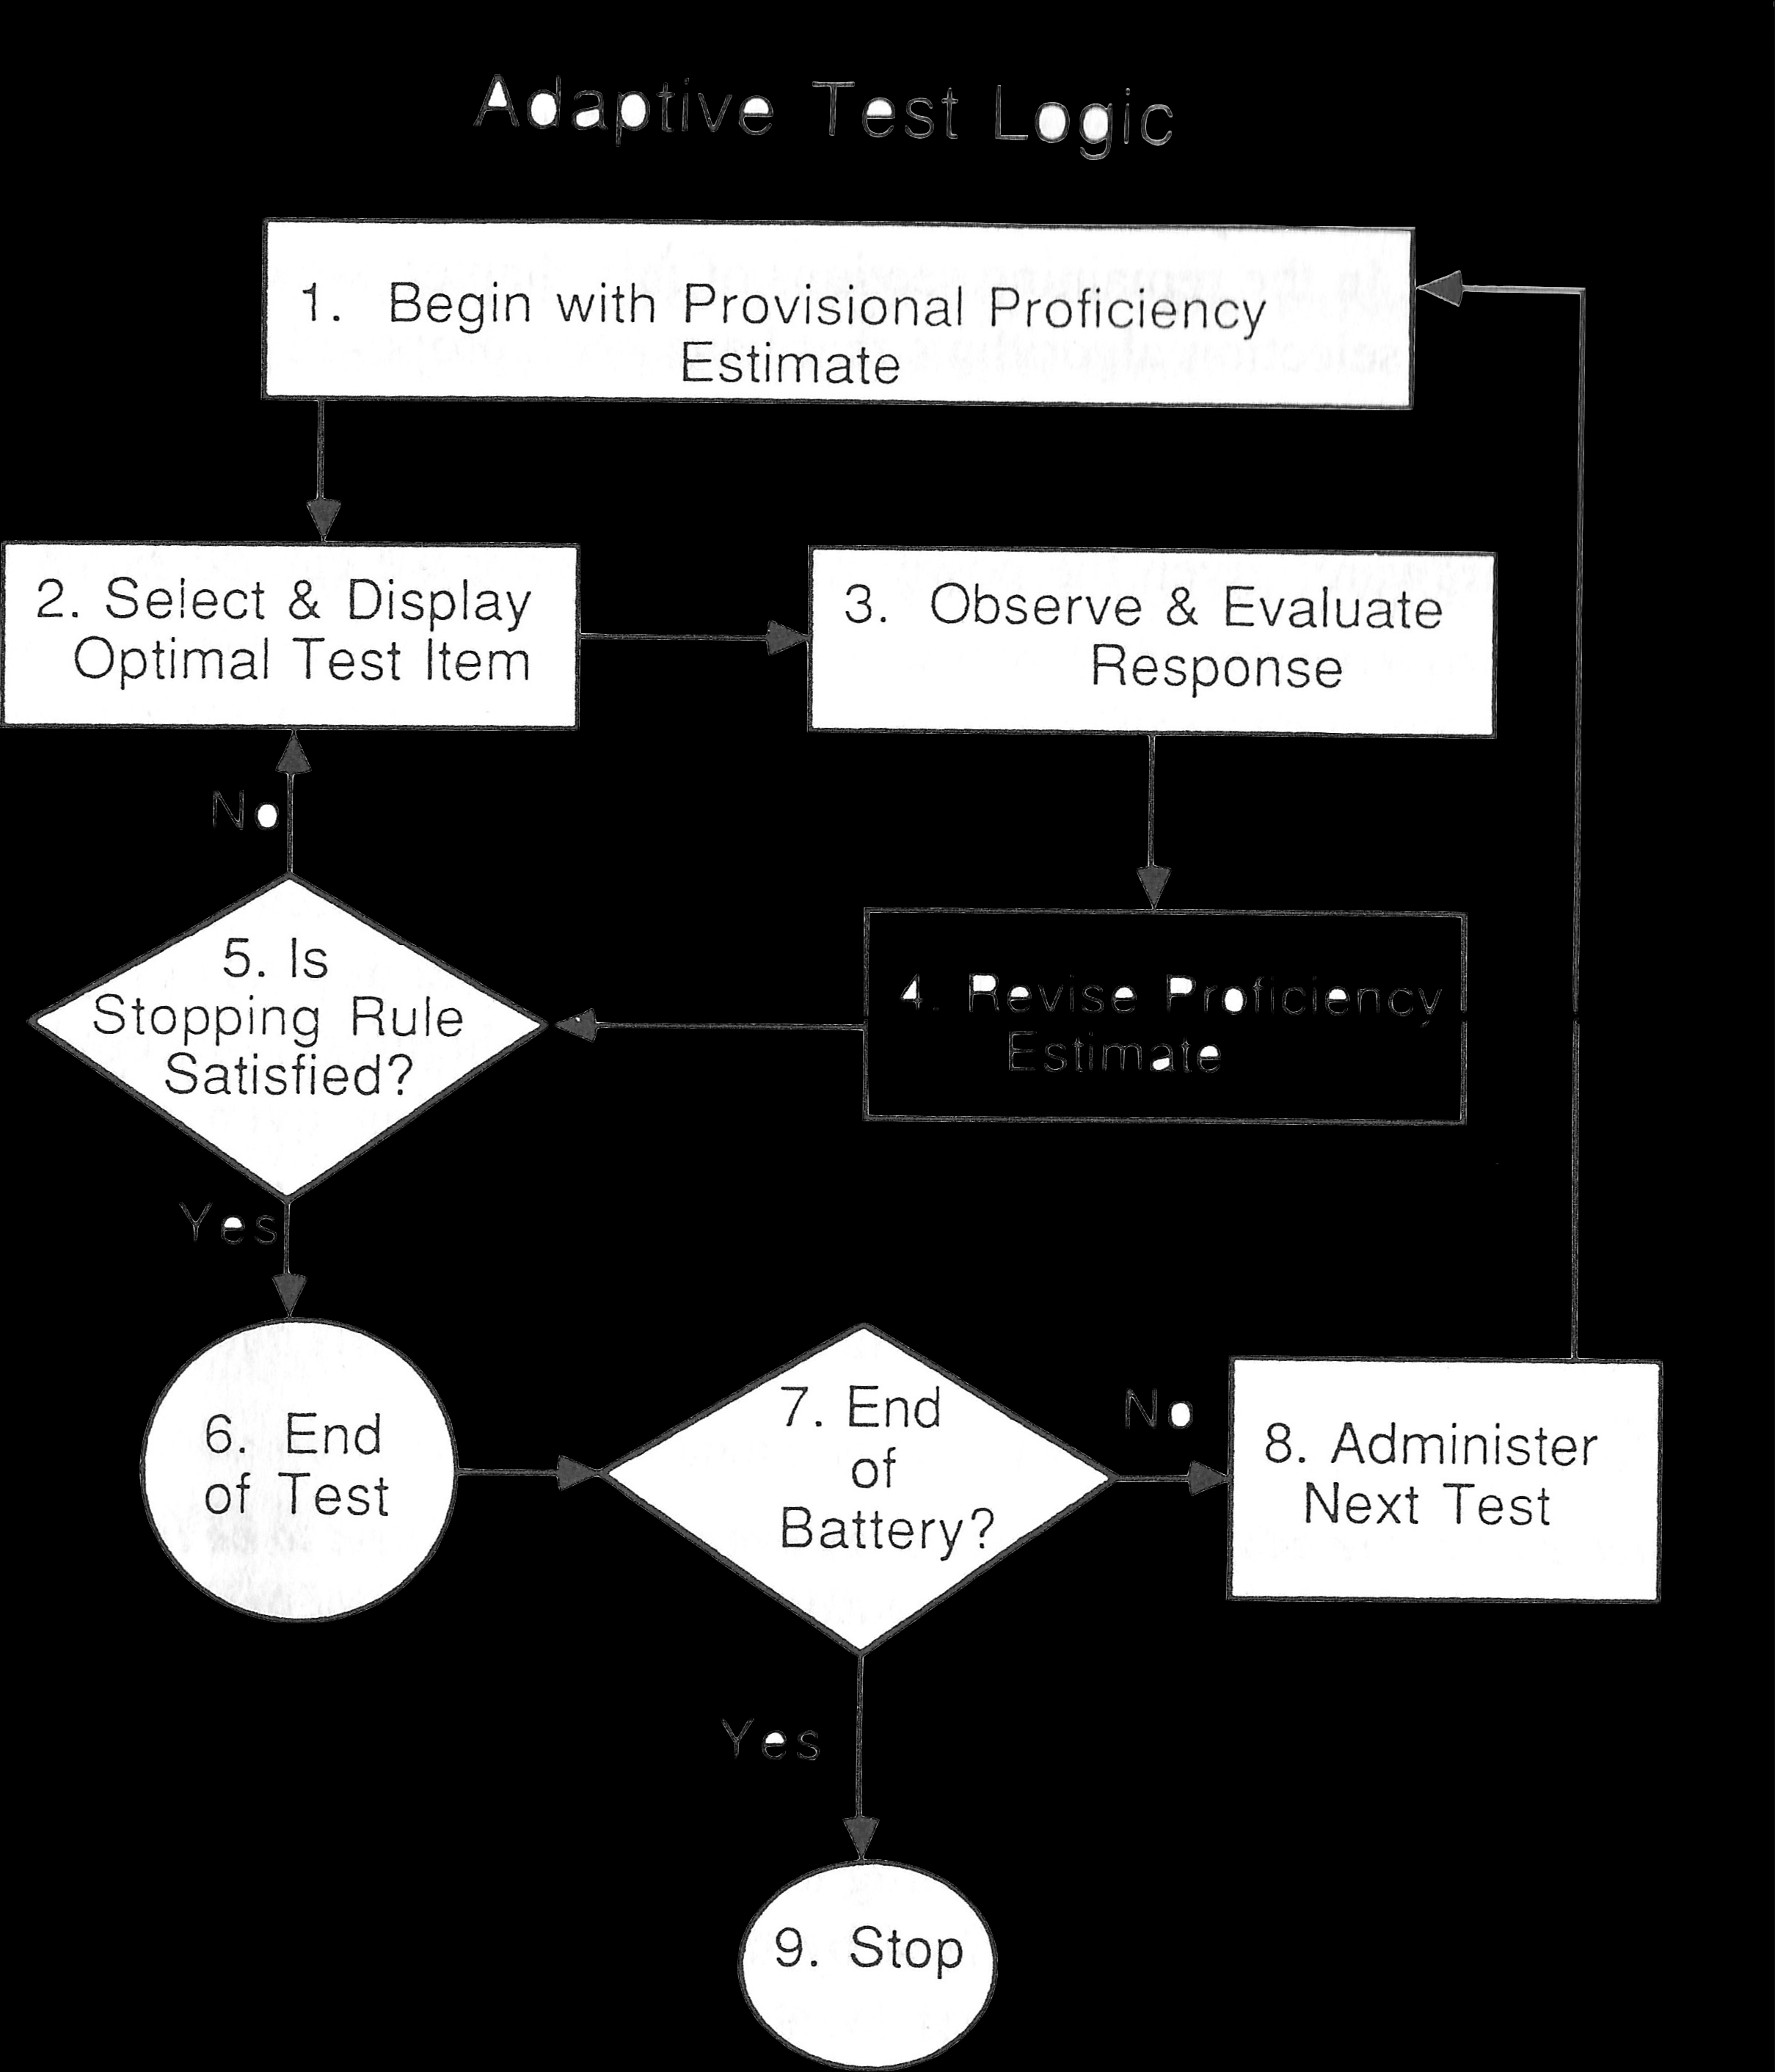
\includegraphics[width=1\textwidth,clip=true]{adaptative_test_logic}
	\caption{Diagrama de flujo de un \acrshort{CAT}}
	\label{fig:diagrama_flujo_CAT}
\end{figure}

Un importante salto ocurrió cuando el la década de los 90 se empezo a investigar la adaptación hipermedia (\acrshort{AH}), y más concretamente, la adaptación hipermedia educativa o \acrshort{AEH}.





In that framework, CAT allows seeing the
students as individuals, taking their own characteristics into
account. Typically, CAT systems are able to adapt the items
presented to the student depending on their former answers, often
including some kind of personalized feedback [12].



Constructing quality test with e-valUAM

Technology-Enhanced Learning (TEL) has a growing presence in educational institutions by making use of Computer-Aided Learning (CAL): a keynote practice where teachers and students are assisted by computers in their teaching/learning processes. Under this perspective, the assessment process is one of those issues that can get profit from the use of these practices. Moreover, completely on-line learning environments, like the emergent trends in Massive Open Online Courses (MOOCs) [1], demonstrate the importance of using CAL environments.

We can find in the literature several examples of assessment tools for some specific learning domains that can give useful and interactive advices to the students [3] [4] [5] [6]. In the context of providing feedback and advice to the students for widespread domains, Computer Adaptive Testing (CAT) provides advantages apart from an instantaneous scoring [7]. 



%
% Diseño y desarrollo
%
\chapter{Diseño y desarrollo\label{sec:disenhoYDesarrollo}}

%\textbf{Rápida intro.}

%En esta sección se presentan los resultados de las fases de análisis de requisitos, diseño y desarrollo realizadas para el proyecto.
%
%Al ser un proyecto asociado a una investigación que se ha desarrollado en varias fases, se consideró que una mejor metodología que se podía utilizar era una basada en el modelo en espiral descrito en \cite{Boehm86} . A pesar de que la metodología presenta varias iteraciones en cada fase, aquí se presentan los resultados agrupados.

En esta sección se presentan los resultados del análisis, diseño y desarrollo del proyecto. Primero, se detallarán todos los requisitos, funcionales y no funcionales, que se han identificado. A continuación, algunas notas sobre el diseño ideado para el proyecto. Para terminar la sección, se detallan aquello más relevantes de la fase de desarrollo.

Como este proyecto nació asociado a una investigación, no se ha utilizado una metodología en cascada clásica, sino un modelo en espiral, partiendo del descrito en \cite{Boehm86}. A pesar de que el modelo describe varias iteraciones, en esta sección se presentan agrupados los resultados a los que se han llegado entre todas las iteraciones.

%TODO: Demostrar todo el dominio que pueda sobre cuestiones de la carrera.

\section{Análisis de requisitos}

Los requisitos aquí detallados son el fruto de un análisis a priori sobre qué necesidades tenía que cubrir el sistema más carencias que se han detectado al ser utilizado en entorno reales y que se han ido añadiendo. Algunas de las mejoras posibles se han detectado en la última iteración realizada y por lo tanto aún no están implementadas. Aún así, están recogidas en el apéndice \ref{apen:analisis de requisitos}. 

\subsection{Análisis funcional}

\begin{rf0}

	\item Gestión de usuarios.
			\begin{rf0*}
				\item El sistema deberá permitir crear cuentas de usuario. Las cuentas tendrán un nombre de usuario y contraseña que identifiquen a cada usuario.
				\item Cada cuenta de usuario tendrá un rol en cada asignatura en la que participe. Podrá ser un rol docente o rol estudiante. Dependiendo del rol que tenga, la cuenta podrá acceder a más o menos funcionalidad en cada sección del sistema, como se detalla más adelante.
				\item El equipo docente de cada asignatura determinará qué alumnos pertenecen a sus grupos.
			\end{rf0*} 

	\item \textbf{Rol docente:} Creación y gestión de materias.
			\begin{rf0*}
				\item Dentro de su asignatura, el docente podrá crear tantas materias como necesite. Cuando cree una materia, deberá establecer un título, el número de niveles en los que se clasificarán las preguntas y el número de respuestas que tendrá cada una.
				\item Una vez creada una materia, el docente podrá modificar su configuración. Podrá cambiar el título en cualquier caso, pero solo podrá cambiar el número de niveles y el número de respuestas cuando no haya preguntas asociadas a la materia o cuando el número aumente. Para disminuir alguno de los dos valores, deberá borrar antes todas las preguntas asociadas a la materia.
			\end{rf0*}

	\item \textbf{Rol docente:} Creación y gestión de preguntas y respuestas.
		\begin{rf0*}
			\item Existiendo al menos una materia, los docentes podrán crear preguntas y respuestas asociadas a dicha materia.
			\item Cuando se cree una pregunta nueva, deberá indicarse la materia a la que pertenece (que deberá haber sido creada previamente), el nivel, el enunciado, la respuesta correcta y el resto de respuestas. El número de respuestas que deberá escribir vendrá condicionado por el valor establecido en la materia relativa.
			\item Opcionalmente, se podrá asociar ficheros multimedia a las preguntas. Se pueden asociar imágenes o audio tanto al enunciado como a cada una de las respuestas. Si se desea asociar un fichero multimedia, deberá especificarse el nombre del fichero.
			\item Opcionalmente, se podrá establecer un mensaje de feecback asociado a la pregunta.
			\item Una vez creada una pregunta, el docente podrá modificar cualquier atributo o borrar dicha pregunta. En ambos casos, se mantendrá una copia en la base de datos de la antigua pregunta para que los alumnos no vean alterados sus cuestionarios una vez realizados.
		\end{rf0*}
	
	\item  \textbf{Rol docente:} Subida y gestión de ficheros multimedia.
		\begin{rf0*}
			\item Existiendo al menos una materia, los docentes podrán subir un fichero de audio (en formato mp3) o imagen (con extensión gif, png, jpeg o jpg) y asociarlo a dicha materia para utilizarlos después en alguna pregunta de la materia.
			\item Se podrá consultar un listado de todos los ficheros multimedia ya subidos a una materia, que mostrará el nombre de cada fichero además de mostrar la imagen o permitir reproducir el audio.
			\item Se podrá actualizar un fichero subiendo otro al servidor con el mismo nombre.
		\end{rf0*}

	\item \textbf{Rol docente:} Creación y gestión de cuestionarios.
		\begin{rf0*}
			\item Existiendo al menos una materia y preguntas suficientes en cada nivel, el profesor podrá crear un cuestionario. Al hacerlo deberá definir un nombre, si el cuestionario será visible a los alumnos, la materia que se usará como banco de preguntas, el número de preguntas que deberán contestarse en cada intento, el tiempo máximo, si el examen acepta respuestas con duda y cómo deberán mostrarse el resultado a los alumnos.
			\item Una vez creado un cuestionario, el docente podrá eliminar el cuestionario. Esto no afectará, en ningún caso, a la información almacenada sobre los cuestionarios ya respondidos por alumnos.
			\item Los docentes podrán acceder a un listado de todos los cuestionarios ya creados.
		\end{rf0*}
		
	\item Realización de cuestionarios.
		\begin{rf0*}
			\item Una vez creado un cuestionario por un profesor, y si está marcado como visible, los alumnos podrán acceder a él.
			\item Una vez que un estudiante acceda a un cuestionario, se le irán mostrando preguntas que deberá ir contestando. Las preguntas se mostrarán en función de las respuestas previas y los niveles establecidos por el profesor.
			\item Si las preguntas van asociadas a ficheros multimedia, estos se mostrarán al estudiante mientras responde. Si aceptan la opción de responder con duda, el alumno tendrá a su disposición un método de establecer que ha respondido con duda.
			\item Para cada pregunta que el alumno responda, quedará almacenado en el sistema a qué cuestionario pertenece, cuando se responde, qué pregunta se ha formulado y cuál ha sido la respuesta elegida. Si hubiera opción de duda, también se mostrará si se ha dudado o no al responder.
		\end{rf0*}
	
	\item Visualización de resultados.
		\begin{rf0*}
			\item Si el profesor ha establecido que los resultados se muestren al terminar el examen, se mostrará la nota final, todas las preguntas, junto con cuál ha sido la respuesta del alumno para cada pregunta y si esta ha sido correcta. El profesor también puede elegir que solo se muestre la nota, o ninguna información.
			\item Cuando una pregunta tenga una cadena de feedback asociada, se mostrará a los alumnos después de que respondan, junto con si la respuesta ha sido correcta o no.\label{RF:feedback}
			\item \textbf{Rol docente:} Los docentes podrán acceder a un listado con todos los intentos que han realizado cada alumno a cada cuestionario que hayan creado. Para cada cuestionario, podrán ver el detalle de cada uno, es decir, qué preguntas se respondieron, cuál fue la respuestas, si era correcta y el instante en el que se respondió.
		\end{rf0*}
\end{rf0}


\subsection{Análisis no funcional}

\begin{rnf0}
	\item Interfaz y usabilidad
		\begin{rnf0*}
			\item La interfaz que el sistema mostrará al estudiante debe ser intuitiva y fácil de usar para todas las edades. Estudiantes alfabetizados deben ser capaces de elegir un cuestionario y completarlo sin asistencia externa. Una clase de niños que aún no sepan leer debe ser capaz de completar un cuestionario sin asistencia del profesor, después de que este les haya configurado el ordenador para que el cuestionario elegido empiece.\label{RNFusabilidad}
			\item La interfaz para el equipo docente deberá ser fácil de aprender para profesores con o sin conocimientos informáticos avanzados. 
			\item Atendiendo a la diversidad de dispositivos con los que los usuarios trabajan, el sistema debe ser capaz de utilizarse en todos los tamaños de pantalla y para ser utilizado con teclado y ratón o pantalla táctil.
		\end{rnf0*}
	\item Seguridad
		\begin{rnf0*}
			\item Debido al carácter secreto de gran parte del contenido creado por los profesores, el sistema deberá garantizar la no accesibilidad de ese contenido a usuarios no autorizados.
			\item Todo usuario que acceda al sistema debe autentificarse previamente a través de un usuario/contraseña, para asegurar la autoría de las respuestas de los cuestionarios.
			\item La autentificación de los usuarios debe ser segura. En concreto, el sistema no almacenará las contraseñas en la base de datos en texto plano. Deberá utilizar un método que garantize que la contraseña no sea conocida aunque se acceda a la base de datos.
		\end{rnf0*}
\end{rnf0}


%\textbf{¿Detallar un análisis funcional? Sí}

\section{Diseño}

Los sistemas adaptativos pueden abstraerse como una serie de módulos como los descritos en la figura \ref{fig:diagrama_disenno}. 

\begin{figure}[htp!]
	\centering
	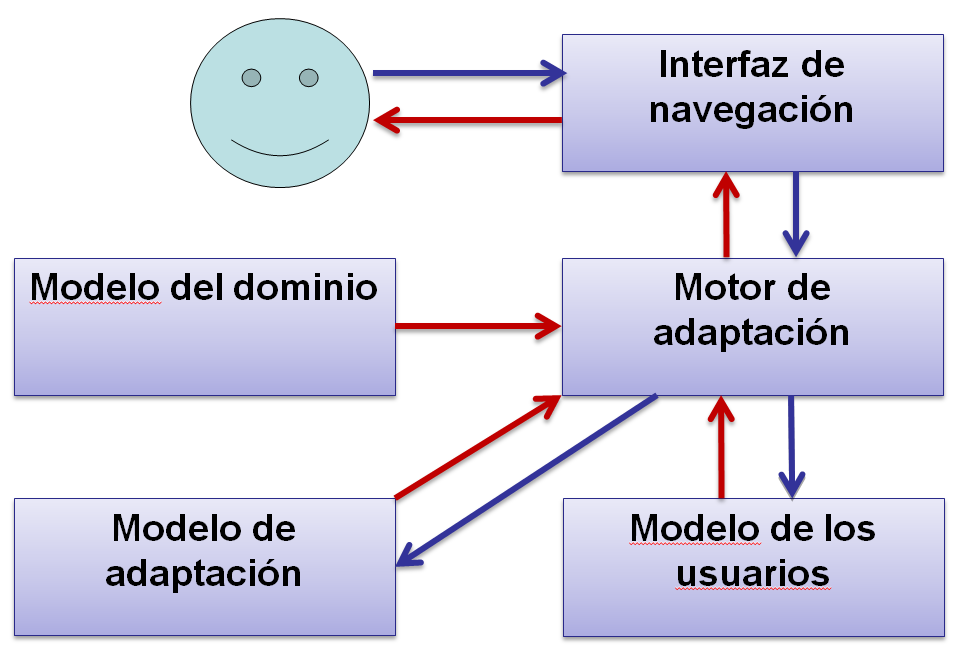
\includegraphics[width=0.75\textwidth,clip=true]{diagrama_disenno}
	\caption{División en módulos de un sistema adaptativo}
	\label{fig:diagrama_disenno}
\end{figure}

El usuario (representado arriba a la izquierda) interacciona con el sistema a través de una interfaz de navegación que representa el estado del motor de adaptación, componente que articula al resto de módulos. El modelo del dominio, de adaptación y el modelo de los usuarios son las herramientas de las que el motor de adaptación obtiene la información que le permite dar una respuesta adecuada a cada situación. Mientras que el modelo del dominio es fijo, en el sentido de que permanece estable durante la vida del mismo, el modelo de adaptación y el modelo de los usuarios van sufriendo variaciones, en función de la entrada que produzcan los usuarios.

Durante las siguientes secciones se dará una descripción más detallada de los módulos.

\subsection{Interfaz de navegación}

La interfaz de navegación es la parte del sistema encargada de permitir la interacción entre el sistema y el usuario. Debe representar ante el usuario la información del sistema que este deba conocer, además de recibir la entrada que el usuario genere para que el motor de adaptación pueda incorporarla.

En el diseño seguido para este trabajo se decidió utilizar las tecnologías web como base sobre la que construir, por lo que las funciones de la interfaz de navegación recaen principalmente en el navegador web del usuario. Aún así, el sistema debe crear y, sobre todo, adaptar los ficheros html que envía al navegador del cliente. Para ello se han utilizado las tecnologías web estándar: HTML, Javascript, CSS y PHP. Más información sobre las tecnologías utilizadas en \ref{sec:tecnologias}.

\subsection{Modelo de los usuarios}

%\textbf{Profesor y estudiante}

El sistema tiene dos roles de usuarios claramente diferenciados: rol docente y rol estudiante. Las necesidades que tienen ambos roles respecto de la aplicación, son radicalmente distintas. Mientras que a los docentes se les debe mostrar herramientas para la creación y gestión de cuestionarios, motorización de resultados y recuperación de exámenes, los estudiantes deben acceder a la ejecución de los cuestionarios, a cierta retroalimentación y a sus resultados.

En ninguno de los dos roles podemos presuponer conocimientos informáticos avanzados, como se recoje en \ref{RNFusabilidad}. Además, desde las fases iniciales del proyecto se planteó que el sistema debería ser fácil de usar para docentes y estudiantes de todas las etapas educativas, desde la primera infancia hasta la edad adulta. Al ser una aplicación potencialmente disponible a niños y niñas muy jóvenes, tampoco podemos presuponer que el estudiante sepa leer, debiendo dotar en consecuencia al rol del docente la habilidad de incluir ficheros multimedia con los que suplir dicha carencia.

\subsection{Modelo del dominio}

La aplicación pretende ser una ayuda al aprendizaje y por lo tanto, su dominio es la actividad educativa. Más concretamente, aquellas actividades relacionadas con comprobar, por parte del propio estudiante o de un docente, si el alumno ha adquirido correctamente ciertos conocimientos. Para ello, a grandes rasgos, el equipo docente de una asignatura creará una serie de preguntas y respuestas, agrupadas por su contenido en materias, que utilizará para crear cuestionarios a los que los estudiantes tendrán acceso. Del resultado de dichos cuestionarios, tanto el estudiante como los docentes podrán conocer cómo están realizando su actividad y realizar los cambios que fueran necesarios.

La asignatura es la primera división que se utiliza normalmente en los entornos educativos. Un docente se encarga de unas asignaturas en concreto y los estudiantes van explorando por asignaturas. Así, cada asignatura tiene asociados un listado de usuarios, algunos comos docentes y otros como estudiantes. Es importante notar que un usuario podría ser docente en una asignatura pero estudiante en otra, por lo que el rol es un atributo de la unión usuario y asignatura, y no solo del usuario.

Dentro de cada asignatura, existen una serie de materias, que son las entidades que clasifican los conocimientos por similitud dentro de una asignatura. El concepto de materia en este modelo se utiliza para representar los conceptos del lenguaje común de \emph{temas} o \emph{partes} en los que se divide una asignatura. Dentro de cada materia existe un conjunto de preguntas, ordenadas por un nivel de relevancia.

La división de las preguntas en niveles de relevancia es una de las características novedosas del modelo propuesto. Con ello se busca facilitar que el estudiante adquiera los conocimientos en el orden más adecuado, asegurando que no se enfrenta a conceptos que dependen de otros hasta que domina los conceptos base. Esta división también ayuda a evitar que un estudiante obtenga una buena calificación en un examen porque haya aprendido a realizar los ejercicios, pero aún así carezca de entendimiento sobre los conceptos básicos. Una discusión más detallada sobre el sistema de clasificación de las preguntas en niveles puede encontrarse en el apéndice \ref{apend:preguntas en niveles}.

Cada pregunta lleva asociada una serie de respuestas y solo una es la válida. Tanto las preguntas como las respuestas llevan asociadas mucha información, como el enunciado, imágenes opcionales\ldots En la figura \ref{fig:modelo del dominio} se encuentran detallada toda la información asociada a cada entidad que compone el modelo.

\begin{figure}[htp!]
	\centering
%	\includegraphics[width=0.75\textwidth,clip=true]{modelo_dominio}
	\caption{Modelo del dominio}
	\label{fig:modelo del dominio}
\end{figure}

Una vez escrito un número suficiente de preguntas, el equipo docente puede crear cuestionarios. Las cuestionarios pueden ser de autoevaluación para los alumnos o de evaluación clásica, aunque para el sistema son casos idénticos.

%\textbf{Estructura de la BD}

\subsection{Modelo de adaptación\label{sec:modelo adapatacion}}

El sistema contempla dos tipos de adaptación. Primero, tenemos la adaptación de navegación, que es aquella que busca guiar al usuario por el sistema, facilitando su uso. En nuestro caso, la navegación del estudiante es sencilla, por lo que no aplica. Donde sí que es necesario este tipo de adaptación es en el área del docente. A la hora de crear las materias, las preguntas y los cuestionarios existe un orden de trabajo más sencillo que otros y el sistema deberá guiar al usuario por ese recorrido utilizando elementos variables de la interfaz.

El otro tipo de adaptación, la adaptación del contenido, es la más relevante para el sistema. Al igual que la de navegación afecta principalmente al docente, la de contenido afecta sobre todo al estudiante. Las preguntas a las que un estudiante se enfrenta en un cuestionario depende de las respuestas que haya dado a las anteriores.

En concreto, cuando un docente crea un cuestionario establece dos parámetros, $N_l$, que es el número de niveles en los que una pregunta se puede clasificar y $N_v$, que es el número de preguntas que debe responder cada alumno en cada intento del cuestionario. Todos los estudiantes empiezan respondiendo a preguntas del primer nivel y solo se enfrentarán a preguntas de niveles más avanzados cuando hayan respondido correctamente a suficientes preguntas. En concreto, a $\frac{N_v}{N_l}$ preguntas.

\begin{figure}[htp!]
	\centering
	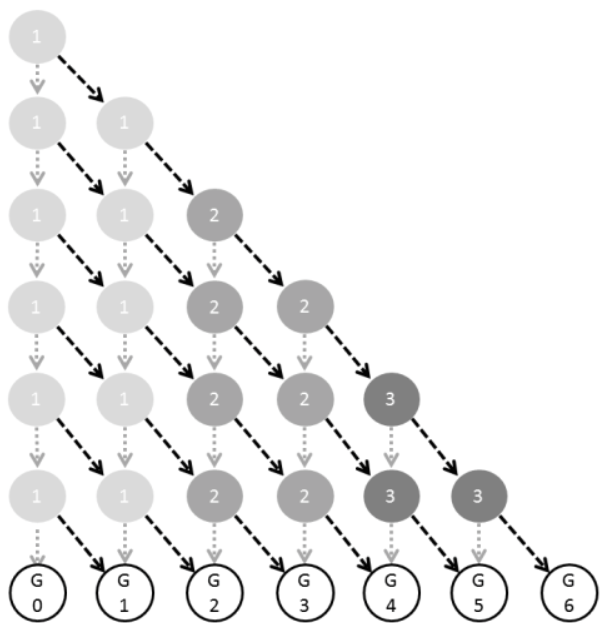
\includegraphics[width=0.5\textwidth,clip=true]{modelo_adaptacion}
	\caption[Modelo de adpatación]{Diagrama que representa todos los posibles recorridos para un cuestionario con $N_l = 3$ y $N_v = 6$. Todos los alumnos entran por la pregunta de la esquina superior izquierda. El número dentro de las circunferencias representa la dificultad de la pregunta. Cuando un alumno responde, toma el camindo de la flecha oscura cuando acierta y de la flecha clara cuando falla. La última fila del diagrama representa las posibles notas que un estudiante puede sacar, ordenadas de menor a mayor de izquieda a derecha.}
	\label{fig:modelo de adaptacion}
\end{figure}

La elección de la siguiente pregunta dentro de un mismo nivel se hace de forma aleatoria, asegurando en todo momento que no haya preguntas repetidas dentro del mismo cuestionario. Cuando el alumno sube de nivel, ya solo responde a preguntas de ese nuevo nivel. Como el número de preguntas está limitado, es posible que un estudiante no llegue a responder preguntas de todos los niveles o incluso puede que solo responda preguntas del primer nivel. Una vez que se ha subido de nivel, no se puede bajar, aunque cada vez que se repita el cuestionario se volverá al primer nivel.

Que la respuesta de una pregunta condicione la siguiente pregunta obliga a que el estudiante responda a cada pregunta, a diferencia de los cuestionarios clásicos, donde una pregunta puede dejarse sin respuesta y continuar con la siguiente. Para solucionar esta diferencia el equipo docente puede establecer que exista una opción adicional de respuesta que indique que el alumno no conoce la respuesta. Si marca está opción, el sistema la tratará como respuesta incorrecta a la hora de seleccionar la siguiente pregunta. Así mismo, la aplicación da al docente la opción de mostrar una casilla que especifique que el alumno ha respondido sin estar seguro de que sea la respuesta correcta. Más información sobre el modelo del examen, en concreto sobre el sistema de calificación, puede encontrarse en el apéndice \ref{apen:como se ponen las notas}

Por último, el docente puede decidir que los estudiantes reciban feedback al responder una pregunta o no, como se describe en \ref{RF:feedback}.


%\textbf{Exámenes con distintos niveles y cómo se pasa de uno a otro. Hablar también del feedback o del no lo sé}



% Susection a ignorara
%\subsection{Motor de adaptación}

%\textbf{Rápidas notas sobre la aplicación en sí. O no.}


\section{Desarrollo: e-valUAM\label{sec:desarrollo}}

En esta sección se detalla cómo se han plasmado los requisitos y el diseño del proyecto en la plataforma online creada, e-valUAM, tomando como referencia lo expuesto en las secciones anteriores del presente capítulo.

\subsection{Visión general}

e-valUAM es el sistema web de creación y respuesta de cuestionarios para ayuda al aprendizaje en el que se ha plasmado este proyecto. Es un sistema que ha sido desarrollado para servir como herramienta de una investigación que viene existiendo desde los últimos tres años, tomando su forma definitiva especialmente en el último año. Para cada año académico se construyó un prototipo diferente que siempre fue una ampliación del prototipo anterior, siguiendo un modelo de desarrollo en espiral.

Al tratarse de parte de una investigación en desarrollo existen algunos requisitos y cuestiones del diseño que se han detectado y recogido, pero que aún no se han implementado. Aún así, todo lo descrito en las secciones anteriores ha sido ya recogido como funcionalidad del sistema.

Además, esta sección está complementada por la información disponible en los apéndices \ref{apen:estructura proyecto} y \ref{apen:codigo}, que hacen referencia a cómo está estructurado el código del proyecto y las partes del código más relevantes, respectivamente.

Por último, y puesto que el sistema requiere de autentificación para poder ser explorado, se ha creado una cuenta a tal propósito cuyo nombre de usuario y contraseña son \textit{TFG}. El sistema está disponible en \url{http://sacha.ii.uam/e-valUAM} y la cuenta aquí especificada tiene permisos tanto de alumno como de profesor, por lo que se pueden explorar libremente todo el sistema.

\subsection{Tecnologías y lenguajes empleados\label{sec:tecnologias}}

Al ser un sistema web, los lenguajes principales son aquellos relacionados con las tecnologías web. En concreto, se ha utilizado HTML5, CSS3 y Javascript para la parte del cliente, mientras que en el servidor se ha utilizado PHP 5. Para el desarrollo de la interfaz de usuario se han utilizado las librerías de Bootstrap 3 y jQuery.

En el lado del servidor se ha utilizado una máquina alojada en la UAM, con sistema operativo Windows 7, servidor Apache 2.2 y como gestor de base de datos PostgreSQL 9.3.

Como editor de código se ha utilizado Sublime Text 3. Para el control de versiones git y como repositorio central, Github.

\subsection{Módulos asociados al docente}

Las cuentas que dispongan de permisos de profesor pueden gestionar sus cuestionarios a través de la zona de profesor, accesible desde \url{http://sacha.ii.uam.es/e-valUAM/profesor/}. Esta sección se divide en 5 módulos principales:

\begin{itemize}
	\item Materias
	\item Preguntas
	\item Exámenes
	\item Ficheros multimedia
	\item Recuperación de exámenes
	%\item Análisis de resultados
\end{itemize}

A continuación se repasarán las características y el funcionamiento de cada uno de ellos.

\subsubsection{Materias, Preguntas y Exámenes}

Los módulos de materias, preguntas y exámenes son los encargados de permitir al usuario crear y gestionar las materias, preguntas y cuestionarios, respectivamente. Los tres tienen un funcionamiento muy parecido, similar al mostrado en la figura \ref{fig:e-valUAM interfaz profesor}.

\begin{figure}[htp!]
	\centering
	\includegraphics[width=1\textwidth,clip=true]{e-valUAM_preguntas}
	\caption{Interfaz de e-valUAM para el profesor}
	\label{fig:e-valUAM interfaz profesor}
\end{figure}

A través del menú superior, al docente puede acceder a todas las secciones de la página. Al entrar en ``Materias'', ``Preguntas'' o ``Exámenes'' verá una interfaz dividida en dos zonas. 

La zona primera (a la izquierda en la imagen, arriba si se accediera desde un dispositivo con una pantalla pequeña) es la que sirve para crear una nueva entidad en el sistema. Un formulario solicita al usuario toda la información relevante. Al pulsar en el botón de ``Guardar'', si con Javascript se comprueba que todos los campos necesarios han sido rellenados, se envía al servidor. En el servidor un fichero PHP recibe la información, la valida y si todo es correcto, la almacena en la base de datos.

La segunda zona (a la derecha en la imagen, al final de la página se se accede con una pantalla pequeña) es donde se lista la información ya almacenada en la base de datos. En formato tabular se muestran todas las entradas. A la izquierda del todo se muestran dos botones para editar la información y borrarla.

Cuando se edita un elemento, aparece un formulario en primer plano con la información almacenada hasta el momento y la posibilidad de establecer un nuevo valor para cada campo. Al final del formulario se ofrecen dos botones, para guardar los cambios o descartarlos sin alterar la base de datos.

\begin{figure}[htp!]
	\centering
	\includegraphics[width=0.75\textwidth,clip=true]{e-valUAM_edicion}
	\caption{Menú de edición para un elemento}
	\label{fig:e-valUAM edicion profesor}
\end{figure}

Si el usuario guarda los cambios, el navegador del usuario envía una petición AJAX con la información del cambio, que es comprobado y procesado por un fichero PHP en el servidor. El servidor responde si se ha podido realizar el cambio o no, para avisar al usuario en caso de que se produjera un error. Si se intenta borrar el elemento, el sistema pedirá confirmación y lanzará una petición AJAX al servidor siguiendo el mismo proceso.

\subsubsection{Ficheros multimedia}

Pensando en hacer la aplicación más accesible a usuarios de corta edad, se incluyó la posibilidad de que la aplicación pudiera incluir imágenes o audio para complementar la información mostrada como texto en las preguntas y las respuestas.

Para poder trabajar con dichos ficheros, la sección de la web dedicada a la web permite a los docentes subir nuevos ficheros o listar los que ya estén. Los ficheros multimedia van asociados a una materia, por lo que lo primero que debe hacerse, tanto para ver como para listar, es elegir con qué materia se quiere trabajar.

Para asegurar la compatibilidad con todos los navegadores modernos el sistema solo acepta imágenes en formatos GIF, PNG o JPEG y audio en formato MP3. Cuando el profesor sube un fichero se guarda en una carpeta en el servidor diferente para cada materia, por lo que cada profesor puede tener sus propios ficheros sin interferir con los demás. En la base de datos, mediante el gestor de preguntas, se asocian los ficheros con las preguntas y las respuestas. Cuando deben mostrarse al usuario, sencillamente el servidor busca el fichero en la carpeta correspondiente para que su navegador se lo muestre al usuario.

\begin{figure}[htp!]
	\centering
	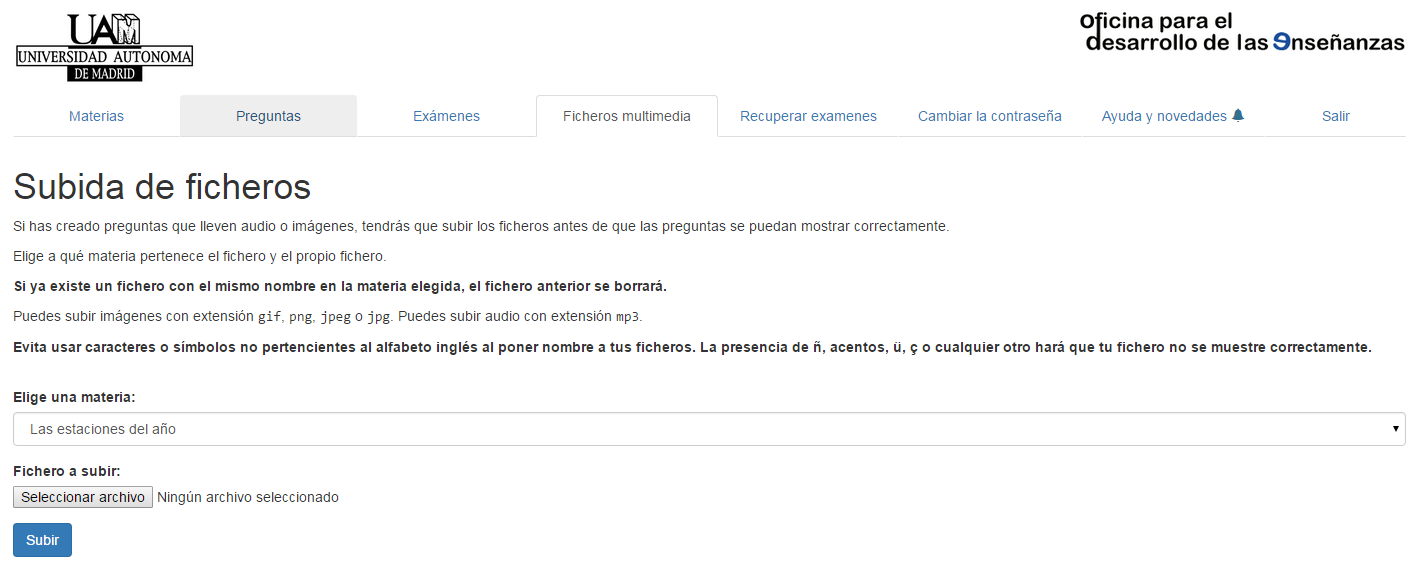
\includegraphics[width=1\textwidth,clip=true]{e-valUAM_multimedia}
	\caption{Subida de ficheros multimedia}
	\label{fig:e-valUAM ficheros multimedia profesor}
\end{figure}

Para que el profesor no tenga que recordar qué ficheros subió o el nombre de los mismos, se incluyó la sección de visión de ficheros. Sencillamente, cuando el docente elige una materia para mostrar, se solicta por AJAX al servidor un listado de todos los ficheros que hay asociados a ella. Cuando el navegador recibe respuesta empieza a mostrarlos si son imágenes o a mostrar un reproductor si se trata de audio.

\begin{figure}[htp!]
	\centering
	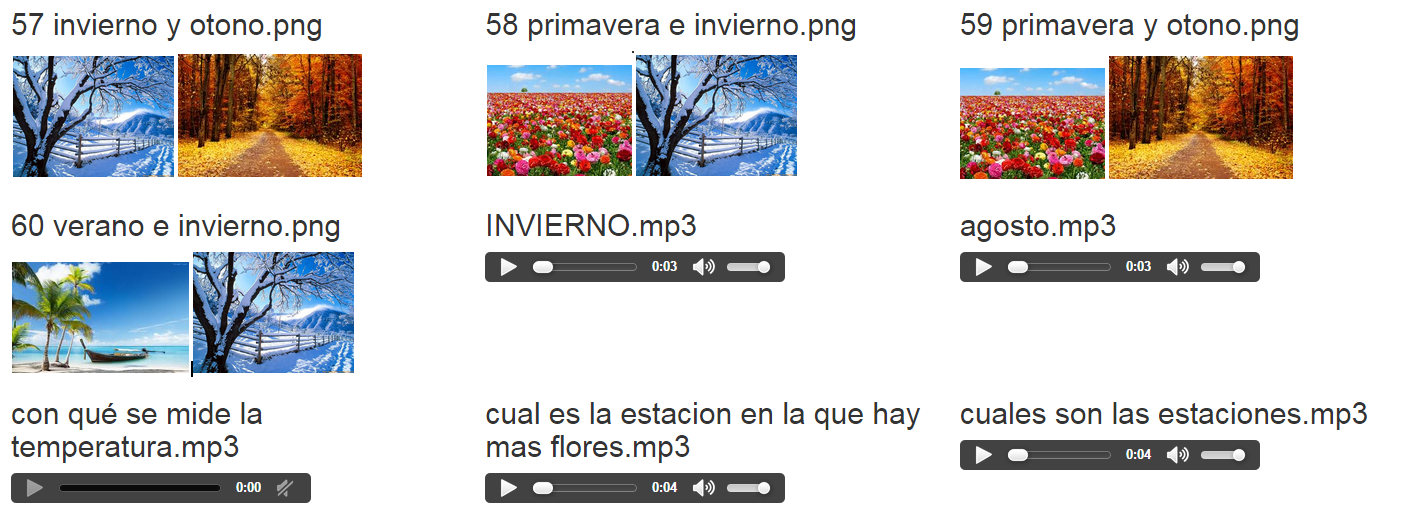
\includegraphics[width=0.75\textwidth,clip=true]{e-valUAM_visor_multimedia}
	\caption{Visor de elementos multimedia}
	\label{fig:e-valUAM visor multimedia profesor}
\end{figure}

\subsubsection{Recuperación de exámenes}

Aunque el sistema realiza una corrección automática de los cuestionarios respondidos por los alumnos, es posible que aún así los profesores deseen revisar los exámenes, ya sea para comprobar personalmente el desempeño de un alumno o para revisar con él sus respuestas o su calificación.

Con ese fin se creó el módulo de recuperación de exámenes. Cuando el profesor lo selecciona en el menú, aparece un listado con todos los cuestionarios que ha creado en algún momento. Cuando selecciona alguno de ellos, gracias a una petición AJAX, se muestra un listado con todos los intentos que ha realizado cada alumno respondiendo a ese cuestionario.

\begin{figure}[htp!]
	\centering
	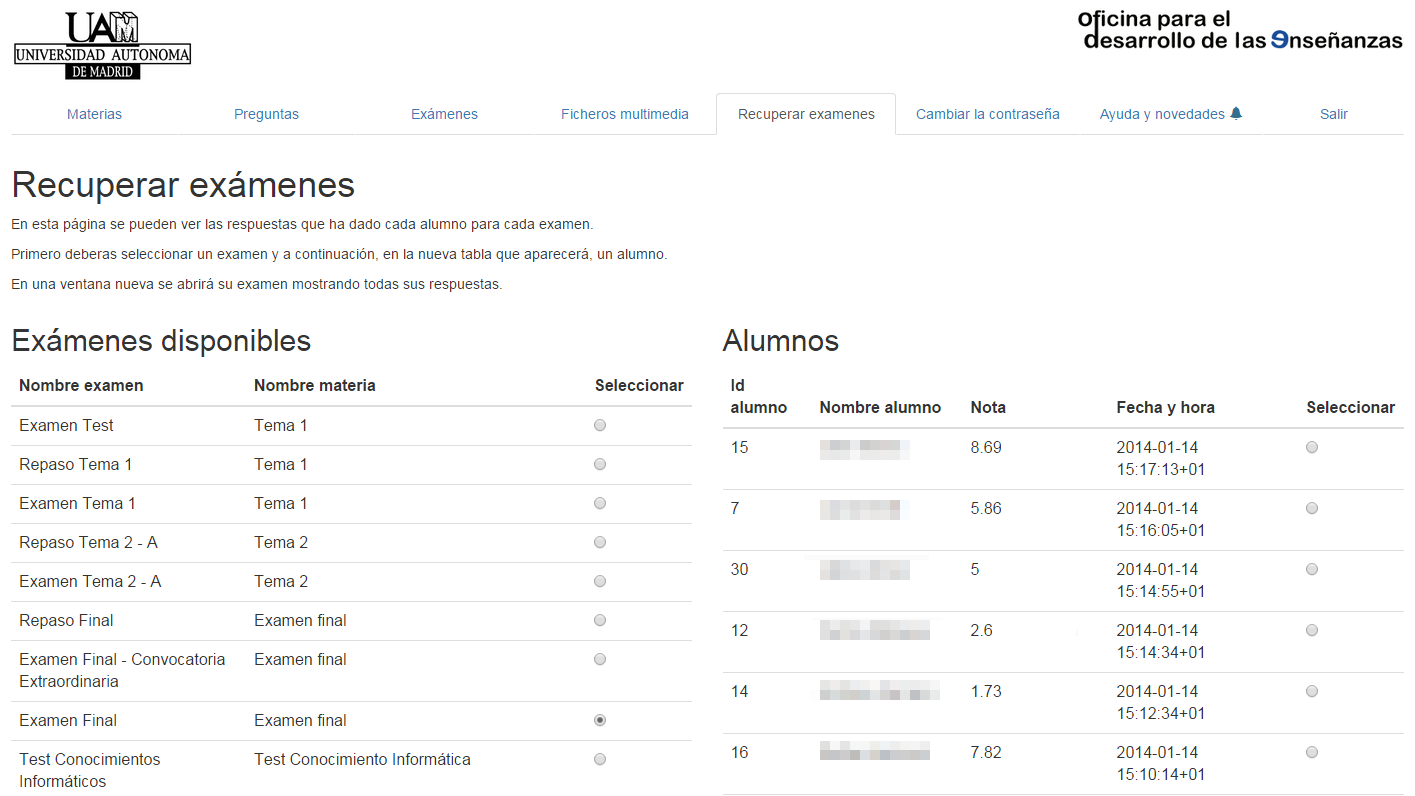
\includegraphics[width=1\textwidth,clip=true]{e-valUAM_recuperacion_examenes}
	\caption[Recuperación de exámenes]{Recuperación de exámenes. Se han difuminado el nombre de los alumnos por respeto a su intimidad.}
	\label{fig:e-valUAM recuperacion examenes profesor}
\end{figure}

Cuando el profesor selecciona un intento en concreto, el sistema muestra ordenadamente todas las preguntas que se eligieron para ese intento, junto a la respuesta que el alumno seleccionó, además de si esta es correcta o no. Para poder realizar esta operación correctamente es por lo que si un profesor modifica una pregunta no se borra de la base de datos, sino que se almacenan ambas versiones, de tal forma que siempre se recupera el examen tal y cómo lo vio el alumno en su momento.

\subsection{Módulos asociados al estudiante}

Las secciones de la página destinas al estudiante son más sencillas y menos abundantes limitándose sencillamente a tres módulos que interaccionan siempre en un orden determinado. Cuando el alumno accede al sistema a través de la página principal, es redirigido a la página de elección de cuestionario, dónde se le ofrecen todos los cuestionarios disponibles para él en ese momento. Una vez que selecciona el cuestionario que desea realizar, este empieza.

\begin{figure}[!htp]
	\subfloat[Respuestas con texto e imagen\label{fig:e-valUAM examen}]{%
		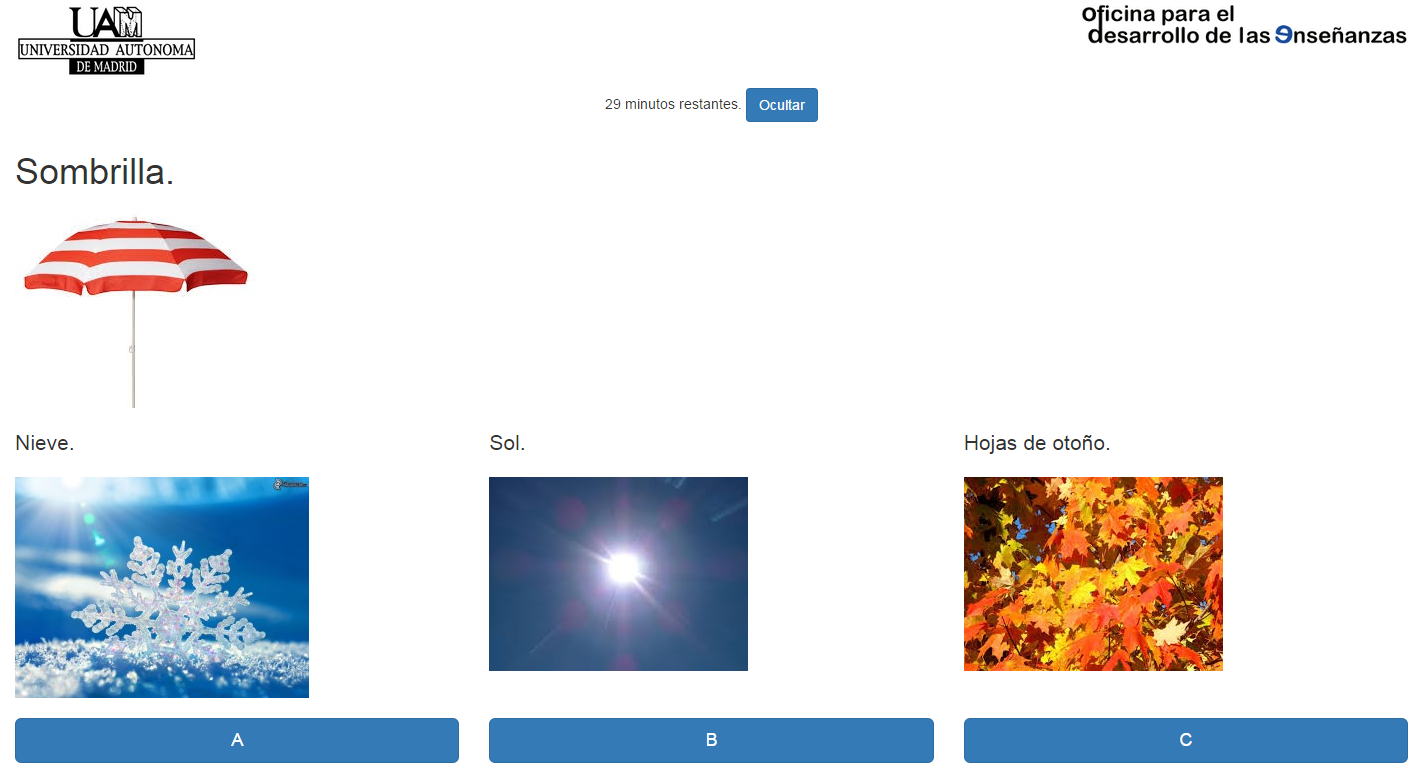
\includegraphics[width=0.45\textwidth]{e-valUAM_examen}
	}
	\hfill
	\subfloat[Respuestas con texto y audio\label{fig:e-valUAM examen audio}]{%
		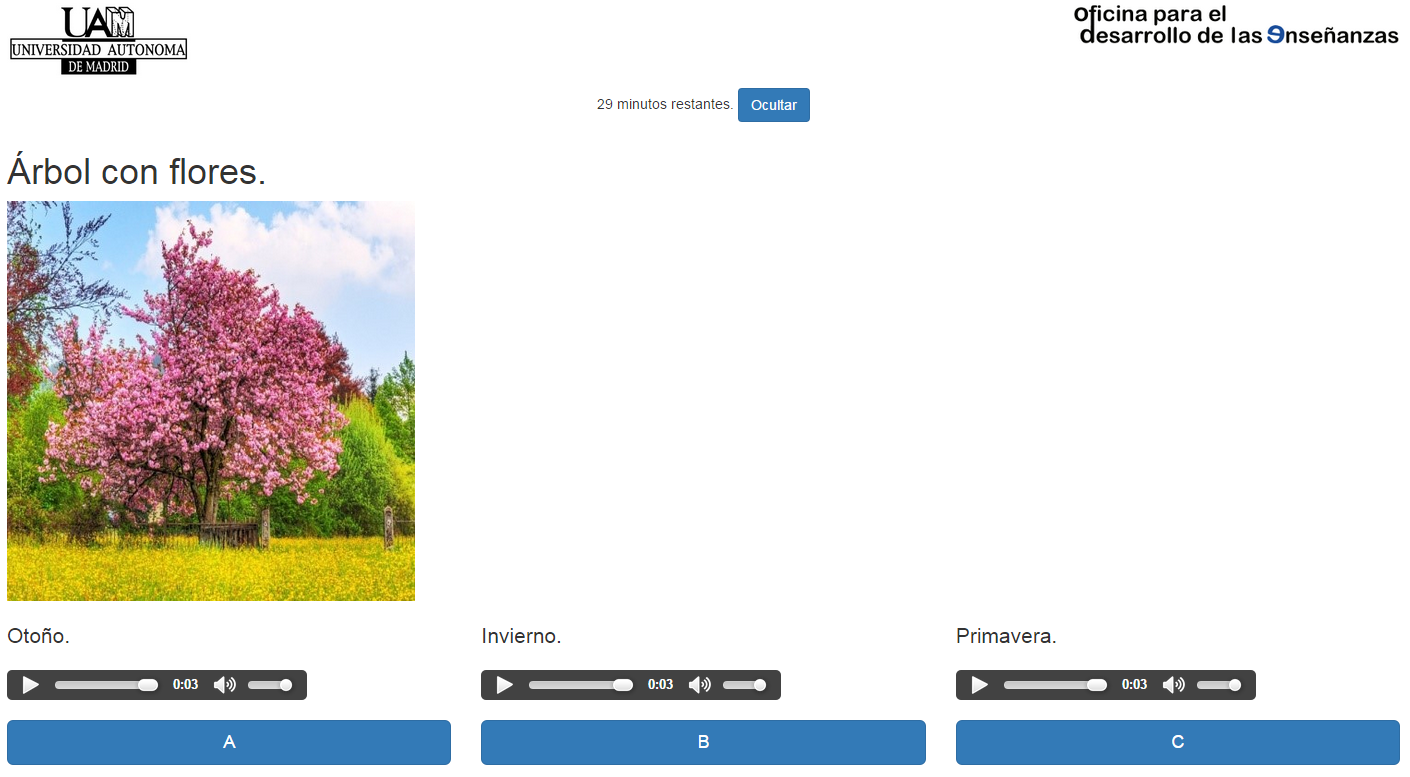
\includegraphics[width=0.45\textwidth]{e-valUAM_examen_audio}
	}
	\caption{Ejemplo de preguntas de un examen}
	\label{fig:e-valUAM examenes}
\end{figure}

Desde ese momento el sistema va seleccionando las preguntas siguiendo el modelo descrito en \ref{sec:modelo adapatacion}. Mientras al alumno aún le queden preguntas por responder y esté dentro del tiempo establecido por el profesor para responder, el examen continuará. Cuando termine con las preguntas o el tiempo, el cuestionario terminará. Dependiendo de qué opción haya elegido el profesor al fijar los parámetros el cuestionario, se mostrará un mensaje indicando que ha terminado el cuestionario, la nota o cada pregunta con la respuesta elegida estableciendo si ha sido correcta o no. A continuación el alumno puede abandonar el sistema o volver a probar con el mismo u otro cuestionario.

%\textbf{En la introducción dejar muy claro qué se ha desarrollado y qué no se ha desarrollado.}



%
% Pruebas y resultados
%
\chapter{Pruebas y resultados\label{sec:pruebasYResultados}}

% IDEAS A VENDER:
% Generalizable y escalable. Podemos cambiar el modelo subyacente sin sufrir
% Meter el apartado de análisis de resultados
% Se han usado por 50 personas y ha aguantado
% Hablar de la base de datos. Del diseño y cómo se ha hecho
% Probado en entorno real

\section{Comparativa con otras soluciones}

\section{2013-2014: Grado en Historia}

Durante el curso académico 2013-2014 los 15 alumnos de la asignatura de ``Historia Antigua I'' en el Grado en Historia de la Universidad Autónoma de Madrid utilizaron e-valUAM como herramienta de estudio y de evaluación.

A lo largo del semestre, los alumnos tuvieron disponibles 3 cuestionarios de autoevaluación y 3 exámenes. La autoevaluación estaba disponible a los alumnos tantas veces como quisieran. De los 15 alumnos, 6 la utilizaron menos de 3 veces, mientras que otros 6 la utilizaron más de 15 veces. 

A lo largo del año, entre tres profesores crearon un total de 372 preguntas, respondiéndose cada una de media unas 12,386 veces.

Los alumnos 

\section{Test sobre conocimientos informáticos}

% Contar que aquí cambiamos el modelo


\section{Caso real. Asignatura en el Grado en Educación Infantil}

\subsection{Aprendizaje}
\subsection{Examen final}
\subsection{Trabajo final}

%
% Conclusiones
%
\chapter{Conclusiones\label{sec:conclusiones}}

A modo de conclusión, a continuación se presentan los \textbf{logros más relevantes} que ha alcanzado el proyecto expuesto a lo largo de todo el documento, con los que se logran satisfacer todos los objetivos que se recogieron en la introducción:

\begin{itemize}
	\item Se ha diseñado un \textbf{sistema adaptativo} inspirado en \textit{Computerized Adaptive Testing} y la \textit{Adaptive Educational Hypermedia} que, utilizando información de modelos de usuarios, de dominio y de adaptación, permite crear cuestionarios personalizados que profesores y alumnos pueden utilizar para medir su rendimiento académico recibiendo de forma instantánea retroalimentación.
	\item Se han desarrollado las herramientas necesarias para que los profesores puedan crear las baterías de preguntas a través de una interfaz online que les abstrae de los modelos subyacentes logrando así que pueda ser utilizada por \textbf{usuarios sin conocimientos informáticos} avanzados.
	\item Se ha diseñado un sistema capaz de trabajar con \textbf{ficheros multimedia} que ofrecen más posibilidades a los profesores a la hora de crear las preguntas. Así mismo, se ha diseñado una base de datos que ha logrado almacenar toda la información sobre el uso, permitiendo análisis posteriores que han llevado a la creación de nuevos modelos y publicaciones científicas.
	\item Se han implementado mecanismos de \textbf{análisis automático} de resultados que permiten detectar a los profesores preguntas defectuosas de forma instantánea para que puedan corregirlas o eliminarlas, simplificando una tarea muy costosa.
	\item Se han construido \textbf{dos prototipos} incrementales y funcionales durante dos años académicos en los cuales han demostrado su flexibilidad, al haber sido probado en ellos varios modelos de adaptación sin que ello haya significado remodelaciones en el resto de módulos.
	\item Ambos prototipos han sido utilizados con éxito en\textbf{ dos entornos reales}, en dos disciplinas distintas y con más de 100 alumnos, habiendo situaciones donde 50 alumnos han utilizado en paralelo el sistema sin que el rendimiento bajara.
\end{itemize}

Por otra parte, aunque todos los objetivos se han cumplido, algunos, como el relativo al análisis de los resultados, podrían beneficiarse de más desarrollo. Así mismo, a lo largo del desarrollo del proyecto han ido surgiendo ideas y propuestas de mejoras del sistema y con todo ello se ha elaborado una lista de retos que desean abordarse en un futuro cercano:

\begin{itemize}
	\item Añadir \textbf{más análisis de resultados}, como remarcar preguntas que tienen un tiempo de respuesta más alto o crear informes con la evolución de cada alumno a lo largo del año o el conjunto agrado de toda la clase. Así mismo, también se desea añadir una biblioteca de gráficos en Javascript (como D3.js) para \textbf{mejorar la visualización} de todos los análisis.
	\item Permitir que se puedan crear \textbf{nuevos tipos de pregunta}, como preguntas de respuesta abierta o preguntas generadas en función a un código especificado por el profesor.
	\item Dar la opción a los profesores de \textbf{elegir qué modelo} de adaptación desean utilizar entre todos los desarrollados.
	\item \textbf{Ampliar} las opciones que ofrecen las herramientas de creación y gestión de materias, preguntas y cuestionarios que tienen accesibles los profesores.
	\item Dedicar esfuerzos en la \textbf{interacción persona-ordenador}. Para ello, se pretende recolectar información sistemática mediante cuestionarios sobre la experiencia de uso a los alumnos que ya lo han probado para solucionar las deficiencias que puedan existir y luego centrar los esfuerzos a hacer que el sistema sea \textbf{accesible} para usuarios con diversidad funcional.
	\item Facilitar las \textbf{tareas de administración} mediante una interfaz web.
\end{itemize}
 

%
% Página en blanco
%
\cleardoublepage

%
% Bibliografía
%
\bibliography{src/bibliografia}
\addcontentsline{toc}{chapter}{Bibliografía}

% No expandir elementos para llenar toda la página
\raggedbottom

%
% Apéndices
%
\appendix
\cleardoublepage
\addappheadtotoc
\appendixpage

%
% TODO: Apéndices del TFG
%
\chapter{Análisis de requisito ampliado\label{apen:analisis de requisitos}}

\begin{rnf0}
	\item Accesibilidad
	\begin{rnf0*}
		\item El sistema debe cumplir con el estándar \acrshort{WCAG} 2.0 en un nivel A.
	\end{rnf0*}
\end{rnf0}

\chapter{Clasificación de las preguntas en niveles. Motivación y metodología\label{apend:preguntas en niveles}}

\chapter{¿Cómo se evaluan los cuestionarios?\label{apen:como se ponen las notas}}


\chapter{Estructura del proyecto\label{apen:estructura proyecto}}

\chapter{Código más relevante\label{apen:codigo}}


%
%\chapter{Ejemplos de bloques y comandos útiles en LaTeX\label{sec:ejemplos}}
%\section{Ejemplo de sección}
%
%
% Breve guía de comandos útiles para la memoria
%
%
% Citar una referencia
%La DARPA creo el protocolo de Internet \cite{ipv4sta}.
%
% Citar un elemento del glosario
%Citamos el acrónimo \gls{FPGA}.
%
% Citar un elemento del glosario (primera letra en may´usculas)
%\Gls{bitstream} es una secuencia de bits.
%
% Insertar una imagen con pie de página
%\begin{figure}[htp!]
%  \centering
%  
\includegraphics[width=0.75\textwidth,clip=true]{Logo_UAM}
%  \caption{Logo de la Universidad Autónoma de madrid.}
%  \label{fig:logo_uam}
%\end{figure} 
%
% Referenciar una etiqueta (label)
%La figura~\ref{fig:logo_uam} se utiliza en la portada.
%
% Nueva página
%\clearpage
%
% Añadir código fuente sin líneas
%\begin{lstlisting}[label=algoritmo:quicksort,language=C,frame=single,caption=Algoritmo de ordenación Quicksort]
%#include <stdio.h>
% 
%void quick_sort (int *a, int n) {
%    int i, j, p, t;
%    if (n < 2)
%        return;
%    p = a[n / 2];
%    for (i = 0, j = n - 1;; i++, j--) {
%        while (a[i] < p)
%            i++;
%        while (p < a[j])
%            j--;
%        if (i >= j)
%            break;
%        t = a[i];
%        a[i] = a[j];
%        a[j] = t;
%    }
%    quick_sort(a, i);
%    quick_sort(a + i, n - i);
%}
%\end{lstlisting}
%
% Bloque de código inseparable
%\begin{code}
%#include <stdio.h>
% 
%void quick_sort (int *a, int n) {
%    int i, j, p, t;
%    if (n < 2)
%        return;
%    p = a[n / 2];
%    for (i = 0, j = n - 1;; i++, j--) {
%        while (a[i] < p)
%            i++;
%        while (p < a[j])
%            j--;
%        if (i >= j)
%            break;
%        t = a[i];
%        a[i] = a[j];
%        a[j] = t;
%    }
%    quick_sort(a, i);
%    quick_sort(a + i, n - i);
%}
%\end{code}
%
% Fórmula dentro de una línea de texto
%La ecuación de Euler ($e^{ \pm i\theta } = \cos \theta \pm i\sin \theta$) es citada frecuentemente como un ejemplo de belleza matemática.
%
% Fórmula independiente
%\begin{equation}\label{eq:pythagoras}
%a^2 + b^2 = c^2
%\end{equation}


% Fin del documento
\end{document}
